\section{background}
\subsection{motivation}
\begin{frame}
    \frametitle{sparse qubit connectivity}
    \begin{itemize}
        \item controlled operations
        \item NISQ architectures:
        \begin{figure}
            \centering
            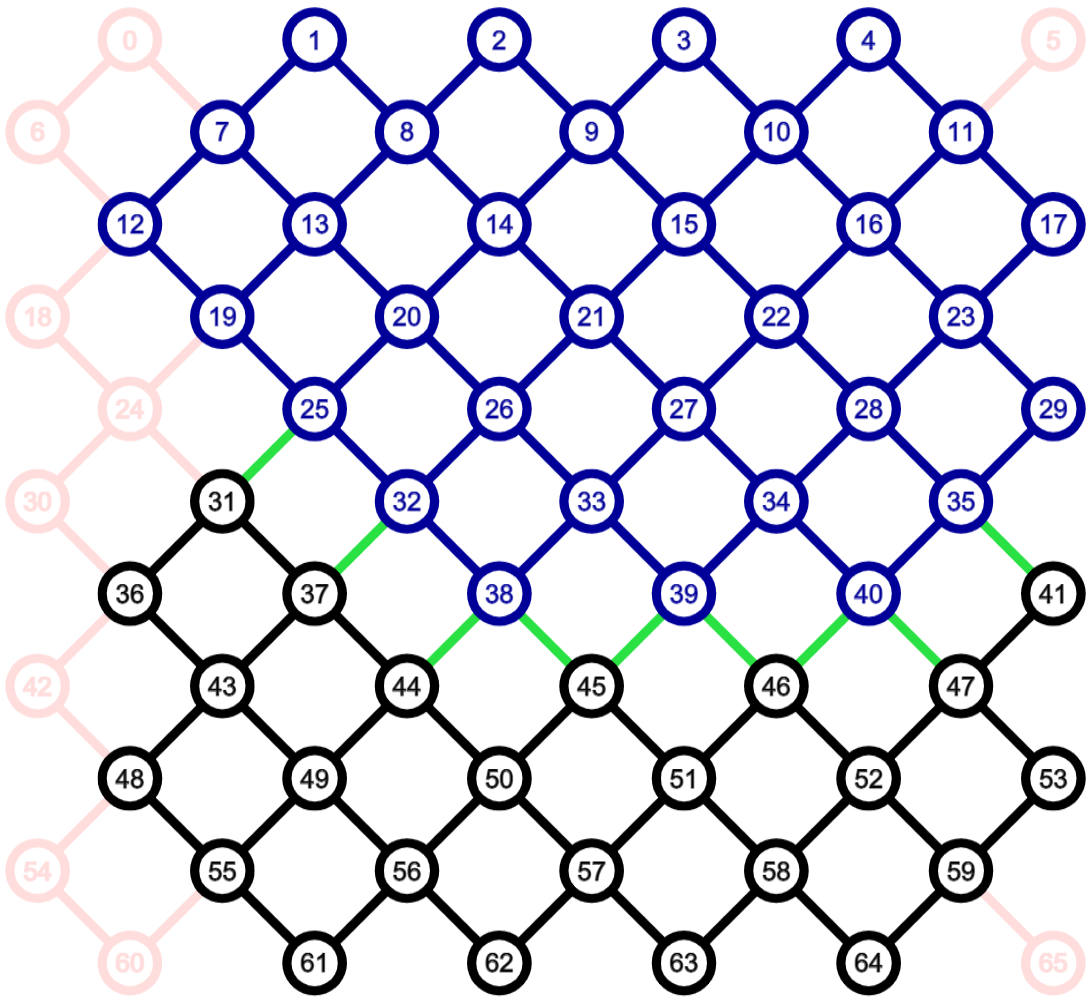
\includegraphics[width=.3\linewidth]{figure/connection.png}
            \caption{Qubit ordering and optimal cut for 56-qubit circuit
            with 20 cycles in \cite{Nash_2020}}
        \end{figure} 
    \end{itemize}
\end{frame}
\begin{frame}
    \frametitle{different sequence of operations}
    \begin{columns}
        \column{0.5\textwidth}
        \begin{minipage}[c][0.4\textheight][c]{\linewidth}
            \centering
            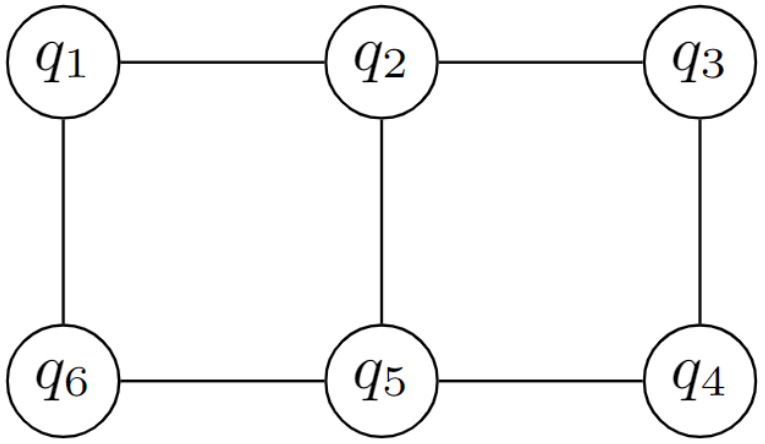
\includegraphics[width=0.8\linewidth]{figure/example.png}
        \end{minipage}
        
        \column{0.5\textwidth} % remember add this to the other clumn
        \begin{minipage}[c][0.4\textheight][c]{\linewidth}
            \centering
            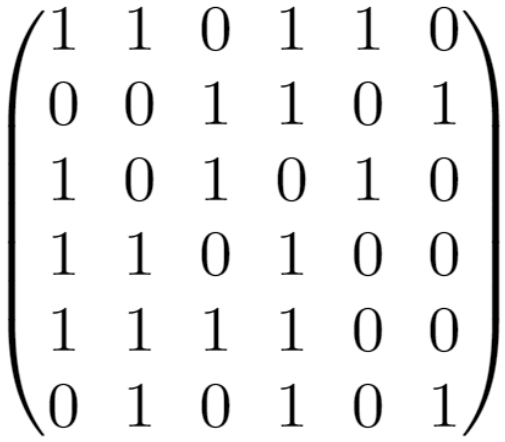
\includegraphics[width=0.8\linewidth]{figure/linear.png}
        \end{minipage}
    \end{columns}
\end{frame}
\subsection{result}
\begin{frame}
    \frametitle{linear reversible circuit synthesis}
    \begin{itemize}
        \item input: the qubit connectivity graph and a binary matrix
        \item $O\left(\frac{n^{3}}{\log {n}} \right)$ VS $O\left(n^{2}\right)$
        \item universal set
        % TODO: need figure 8
    \end{itemize}
\end{frame}